\documentclass[a4paper,12pt]{article} 
\usepackage{geometry}
\geometry{
	a4paper,
	total={170mm,257mm},
	left=20mm,
	top=20mm,
}
\usepackage{titlesec}
\titlelabel{\thetitle.\quad} %точка в section

%%% Работа с русским языком
\usepackage{cmap}                           % поиск в PDF
\usepackage{mathtext} 			 	       % русские буквы в формулах
\usepackage[T2A]{fontenc}               % кодировка
\usepackage[utf8]{inputenc}              % кодировка исходного текста
\usepackage[english,russian]{babel}  % локализация и переносы

%Математика
\usepackage{amsmath,amsfonts,amssymb,amsthm,mathtools} % AMS
\usepackage{icomma} % "Умная" запятая

%% Шрифты
\usepackage{euscript}	 % Шрифт Евклид
\usepackage{mathrsfs} % Красивый матшрифт

%% Команды
\DeclareMathOperator{\const}{\mathop{const}}

%% Перенос знаков в формулах
\newcommand*{\hm}[1]{#1\nobreak\discretionary{}
	{\hbox{$\mathsurround=0pt #1$}}{}}

%%% Заголовок
\author{Шерхалов Денис Б02-204}
\title{Лабораторная работа 2.5.1 \\
	\textbf{Измерение коэффициента поверхностного натяжения жидкости}}
\date{\today}

\begin{document}
	
	{\Large \maketitle}

	\paragraph*{Цель работы:} 1) измерение температурной зависимости коэффициента поверхностного натяжения дистиллированной воды с использованием известного коэффициента поверхностного натяжения спирта;  2) определение полной поверхностной энергии и теплоты, необходимой для изотермического образования единицы  поверхности жидкости  при различной температуре. 
	\paragraph*{В работе используются:} прибор  Ребиндера с термостатом и микроманометром; исследуемые жидкости; стаканы.
	
	\section{Введение}
	Из-за поверхностного натяжения возникают разные давления с разных сторон искривленной поверхности жидкости:
	\begin{equation}
		\Delta P = P_{внутри} - P_{снаружи} = \frac{2\sigma}{r} \;(формула\; Лапласа)
	\end{equation}
	$\sigma$ - коэффициент поверхностного натяжения, $r$ - радиус кривизны поверхности.
	
	\subparagraph*{Экспериментальная установка:}
	
	\begin{figure}[h!]
	\centering{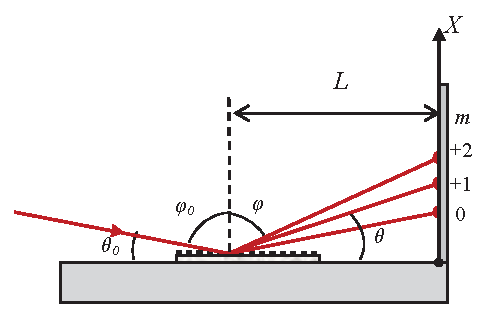
\includegraphics[width=0.75\textwidth]{pic1.jpg}}
	\caption[]{\label{fig:1} Схема установки для измерения температурной зависимости коэффициента поверхностного натяжения}
	\end{figure}

	Схема экспериментальной установки представлена на рисунке 1. Исследуемая жидкость (дистиллированная вода) наливается в сосуд $B$. Тестовая жидкость (этиловый спирт) наливается в сосуд $E$, через пробку в него входит полая металлическая игла $C$. Колбы герметично закрываются. Верхний конец иглы открыт, а нижний погружен в жидкость. При создании достаточно разреженного воздуха в колбе, пузырьки воздуха начинают пробулькивать. Поверхностное натяжение можно определить по величине разряжения $\Delta P$, необходимого для прохождения пузырьков (при известном радиусе иглы).
	
	\quad Разряжение в системе создается с помощью аспиратора $A$. Кран $K2$ разделяет две полости аспиратора. Верхняя полость при закрытом кране $K2$ заполняется водой. Затем кран $K2$ открывают и заполняют водой нижнюю полость  аспиратора. Разряжение воздуха создается в нижней полости при открывании крана $K1$, когда  вода вытекает из неё по каплям. В колбах $B$ и $C$, соединённых трубками с нижней полостью аспиратора, создается такое же пониженное давление. Разность давлений в полостях с разряженным воздухом и атмосферой измеряется спиртовым микроманометром.
	
	\quad Для стабилизации температуры исследуемой жидкости через рубашку $D$ колбы $B$ непрерывно прогоняется вода из термостата. 	Для стабилизации температуры через рубашку колбы с исследуемой жидкостью прогоняется вода из термостата. Из-за большой теплопроводности трубки температура в разных частях трубки заметно различна и ввиду теплового расширения поднимается уровень жидкости при изменении температуры. Поэтому при температурном измерении кончик иглы опускают до самого дна сосуда, тогда:
	\begin{equation}
		\Delta P = P - \rho g h
	\end{equation}
	$\rho$ - плотность жидкости, $h$ - высота погружения иглы.
	

	\section{Выполнение}
	\begin{enumerate}
		\item Проверим герметичность установки. Наблюдение за показаниями манометра показало отсутствие течи в установке 
		
		\item Начнём измерения. Откроем кран К1. Подберём частоту падения капель из аспиратора так, чтобы максимальное давление манометра не зависело от этой частоты (порядка 1 капля в 5 секунд).
		
		\item Измерим максимальное давление $\Delta P_{спирт}$  при  пробулькивании пузырьков воздуха через спирт. 
		$$x_0 = 41.0 \pm 0.5 \, мм \quad \Rightarrow \quad \Delta P_{спирт} = 9.81\cdot0.2\cdot x_0 = 80.4 \pm 1.0 \, Па$$
		Табличное значение коэффициента поверхностного натяжения спирта $\sigma_{сп} = 22.78 \, \frac{мН}{м}$, значит, по формуле (1), диаметр иглы. 
		$$ r = \dfrac{2\sigma_{сп}}{\Delta P} = 0.567\, мм, \quad \Delta r = \dfrac{2\sigma_{сп}\delta P}{\Delta P^2} = 0.007 \, мм$$
		Диаметр иглы, измеренный по микроскопу получился порядка $d = 1.15 \pm 0.05 \, мм$, а значит, косвенное измерение радиуса совпадает с прямым в пределах погрешности.
		
		\item Промоем и просушим от спирта иглу, вставим её в колбу с дистиллированной водой. Измерим максимальное давление $Р_1$ при пробулькивании пузырьков, когда игла лишь касается поверхности воды.  
		$$x_1 = 129.0 \pm 0.5 \, мм \quad \Rightarrow \quad \Delta P_1 = 9.81\cdot0.2\cdot x_1 = 253.1 \pm 1.0 \, Па$$
		Измерим расстояние между верхним концом иглы и неподвижной частью прибора $h_1 = 17.5 \pm 0.5 \, мм$.
		
		\item Утопим иглу до предела (так, чтобы образующийся пузырёк не касался дна). Измерим $h_2 = 7.5 \pm 0.5 \, мм$.
		Измерим максимальное давление в пузырьках $Р_2$.
		$$x_2 = 179.0 \pm 0.5 \, мм \quad \Rightarrow \quad \Delta P_2 = 9.81\cdot0.2\cdot x_2 = 351.2 \pm 1.0 \, Па$$
		По разности давлений $\Delta Р_{12} = Р_2 - Р_1 = 98.1 \pm 1.0 \, Па$ определим глубину погружения иглы косвенно:
		$$\Delta h_{12} = \dfrac{\Delta Р_{12}}{\rho g} = \dfrac{98.1}{998.2\cdot9.81} = 10.0\pm0.1 \, мм$$ 
		Что совпадает с прямым измерением погружения иглы $\Delta h_{12}^{*} = h_1- h_2 = 10.0 \pm 0.5 \, мм$. 
		
		\item Снимем температурную зависимость $\sigma (Т)$ дистиллированной воды. Для этого включим термостат и подождём, пока нужная температура не стабилизируется. После этого проведём измерение давления. (Таблица №1, график №1).
		
		Посчитаем погрешности. Приборные:
		$$\Delta t = 0.1^\circ C,\quad \Delta H = 0.5 \, мм$$
		Далее:
		$$\delta P = 0.2\cdot9.81 \cdot\Delta H \approx 1.0 \, Па,\quad \Delta (\rho gh) = \rho g \Delta h_{12} \approx 1.0 \, Па,\quad \Delta(\Delta P) = \frac{1}{2}(\delta P + \Delta (\rho gh)) = 1.0 \, Па$$
		$$\Delta \sigma = 0.5\left(\Delta(\Delta P) \, r +  \Delta P \, \Delta r\right) \approx 1.14 \, ^{мН}/_{м}$$
		

		\begin{table}[h!] 
			\caption{Измерение $\sigma (t)$}
			\begin{center}
				\begin{tabular}{|*{7}{l|}}
					\hline
					$t$, $^\circ C$ & $H$, мм & $P$, Па & $\rho_{вода},\;^{кг}/_{м^{3}}$ & $\rho gh,\; Па$ & $\Delta P$, Па & $\sigma$, $^{мН}/_{м}$ \\ \hline
					30.0 & 179 & 351.2 & 995.6 & 97.7 & 253.5 & 71.87 $\pm$ 1.17 \\ \hline
					40.0 & 176 & 345.3 & 992.2 & 97.4 & 247.9 & 70.28 $\pm$ 1.15  \\ \hline
					45.0 & 174 & 341.4 & 990.2 & 97.2 & 244.2 & 69.23 $\pm$ 1.14  \\ \hline
					50.0 & 173 & 339.4 & 988.0 & 97.0 & 242.4 & 68.72 $\pm$ 1.13  \\ \hline
					60.0 & 169 & 331.6 & 983.2 & 96.5 & 235.1 & 66.65 $\pm$ 1.11  \\ \hline
				\end{tabular}
			\end{center}
		\end{table}
	
	
		\begin{table}[h!] 
			\caption{Таблица теоретической зависимости плотности $\rho,\;^{кг}/_{м^{3}}$ от температуры $t,\;^\circ C$ воды и спирта}
			\begin{center}
				\begin{tabular}{|*{4}{l|}}
					\hline
					$t$, $^\circ C$ & $\rho_{вода},\;^{кг}/_{м^{3}}$ & $\rho_{спирт},\;^{кг}/_{м^{3}}$ & $\sigma^*$, $^{мН}/_{м}$ \\ \hline
					30 & 995.6 & 781.0 & 71.20 \\ \hline
					40 & 992.2 & 772.2 & 69.60 \\ \hline
					45 & 990.2 & 767.8 & 68.78 \\ \hline
					50 & 988.0 & 763.3 & 67.94 \\ \hline
					60 & 983.2 & 754.1 & 66.24 \\ \hline
				\end{tabular}
			\end{center}
		\end{table}
	
	
		\begin{figure}[h!]
			\centering{\includegraphics[width=1.0\textwidth]{gr1.png}}
			\caption[]{\label{fig:2} График №1}
		\end{figure}
	
	
		\item По графику найдём температурный коэффициент $\dfrac{d\sigma}{dT} = -0.17 \pm 0.07\, ^{мН}/_{м^\circ C}$
		Для нахождения погрешности проведём прямую МНК (красный цвет) и крайние варианты (серый цвет).
		$$k_{max} \approx -0.10\, ^{мН}/_{м^\circ C}, \quad k_{min} = -0.25\, ^{мН}/_{м^\circ C} \quad \Rightarrow \quad \Delta\left(\dfrac{d\sigma}{dT}\right) = \dfrac{|k_{max} - k_{min}|}{2} = 0.7\, ^{мН}/_{м^\circ C} $$
		Несмотря на сильную погрешность результата, он идеально совпадает с табличным $\dfrac{d\sigma}{dT}^{*} = -0.17\, ^{мН}/_{м^\circ C}$
	
		
		\item Построим теперь график теплоты образования единицы поверхности жидкости от температуры $q = -T\dfrac{d\sigma}{dT}$. (График №2).
	
	
		\item И график поверхностной энергии $U$ единицы площади $F$:  $\dfrac{U}{F} = (\sigma - T\dfrac{d\sigma}{dT})$. (График №3). 
		
\end{enumerate}
	
\section{Вывод}

	В интервале температур от 30$^\circ C$ до 60$^\circ C$ зависимость $\sigma = \sigma(T)$ является линейной с коэффициентом наклона $\dfrac{d\sigma}{dT} = -0.17\,\pm\, 0.07 \, ^{мН}/_{м^\circ C}$. Стоит отметить, что наш результат в пределах погрешности совпадает с табличным значением $\dfrac{d\sigma}{dT} \approx -0.16\, ^{мН}/_{м^\circ C}$. \\
	
	Теплоты образования единицы поверхности жидкости $q = q(T)$ линейно зависит от температуры на исследуемом интервале температур. \\
	
	Внутренняя энергия поверхности $\dfrac{U}{F}$ не зависит от температуры и есть константа $U = 77$ $^{мДж}/_{м^2}$.

		
	\begin{figure}[h!]
		\centering{\includegraphics[width=1.0\textwidth]{gr2.png}}
		\caption[]{\label{fig:3} График №2}
	\end{figure}
	
	\begin{figure}[h!]
		\centering{\includegraphics[width=1.0\textwidth]{gr3.png}}
		\caption[]{\label{fig:4} График №3}
	\end{figure}

\end{document}